\documentclass[11pt]{article}

\usepackage{comment} % enables the use of multi-line comments (\ifx \fi) 
\usepackage[a4paper,margin=1cm]{geometry}
\usepackage[utf8]{inputenc}
\usepackage[ngerman]{isodate}
\usepackage{gensymb}
\usepackage{graphicx}
\usepackage{booktabs}% http://ctan.org/pkg/booktabs
\usepackage{tabularx}
\usepackage{ltablex} % Longtables with tabularx
\usepackage[x11names]{xcolor}
\usepackage{amsmath}
\usepackage{amssymb}
\usepackage{array}
\usepackage{wrapfig}
\usepackage{subcaption}
\usepackage{csquotes}
\usepackage{lscape}
\usepackage{geometry}
\usepackage{multicol}
\usepackage{bm}
\usepackage{enumitem}
\usepackage{hyperref}
\usepackage{mdframed}
\usepackage{scalerel}
\usepackage{stackengine}
\usepackage{mathtools}
\usepackage{pdfpages}

% Code highlighting
\usepackage{minted}
\surroundwithmdframed{minted}

% Be able to caption equations and float them in place
\usepackage{float}

\newmdtheoremenv{theorem}{Theorem}
\geometry{a4paper, margin=2.4cm}

\newcommand\equalhat{\mathrel{\stackon[1.5pt]{=}{\stretchto{\scalerel*[\widthof{=}]{\wedge}{\rule{1ex}{3ex}}}{0.5ex}}}}
\newcommand\defeq{\mathrel{\overset{\makebox[0pt]{\mbox{\normalfont\tiny def}}}{=}}}
\newcolumntype{C}{>{\centering\arraybackslash}X}

\DeclarePairedDelimiter\abs{\lvert}{\rvert}
\DeclarePairedDelimiter\norm{\lVert}{\rVert}

\setcounter{tocdepth}{3}
\setcounter{secnumdepth}{3}

\graphicspath{{./img/}}

\begin{document}
	
\title{Predictive Modelling FS20}
\author{Pascal Baumann\\pascal.baumann@stud.hslu.ch}
\maketitle



For errors or improvement raise an issue or make a pull request on the \href{https://github.com/KilnOfTheSecondFlame/mse_summaries}{github repository}.

\tableofcontents
\newpage



\section{Introduction}
Statistical Modelling means finding a density function that produces your given data.

From Wikipedia: "Predictive modeling uses statistics to predict outcomes. Most often the event one wants to predict is in the future, but predictive modelling can be applied to any type of unknown event, regardless of when it occurred.

In many cases the model is chosen on the basis of detection theory to try to guess the probability of an outcome given a set amount of input data."

Predictive modelling is done with Supervised Models, the major challenge in using data to make predictions is distinguishing what is a meaningful signal from the noise.

\section{Continuous Random Variables}
The set of all possible outcomes of a random experiment is called sample space $\omega$. Random variables $X$ are real-valued functions on $\omega$. $W_X$ is the value range, that is the set of all values which $X$ can take on. If $W_X$ is discrete then $X$ is called a \emph{discrete} random variable. A probability mass function (PMF) is the probability that $X$ takes on a given value and is written as $P(X=k)$, a probability distribution is the cumulative PMF for all values $x$ in $W_X$.

\subsection{Properties of Probability Density Functions}
\begin{enumerate}
	\item $f(x) \geq 0\quad \text{for all }x$
	\item $P(a<X\leq b) = F(b) - F(a) = \int_{a}^{b}f(x) dx\quad \text{area between }a \text{ and }b \text{ under }f(x)$
	\item $ \int_{-\infty}^{\infty}f(x) dx = 1$
\end{enumerate}

\begin{theorem}
	The \textbf{expected value} of a continuous random variable is defined as
	\begin{equation*}
			\text{E}(X) = \int_{-\infty}^{\infty} x\cdot f(x) dx
	\end{equation*}
	The \textbf{variance} of a continuous random variable is defined as
	\begin{equation*}
		\text{Var}(X) = \sigma_X^2 = \text{E}((X - \text{E}(X))^2) = \int_{-\infty}^{\infty} (x - \text{E}(X))^2 f(x) dx = \text{E}(X^2) - \text{E}(X)^2
	\end{equation*}
	A \textbf{quantile} $q(\alpha) (0<\alpha<1)$ of a continuous random variable $X$, respectively of a probability distribution is defined as
	\begin{equation*}
		P(X\leq q(\alpha)) = \alpha \Leftrightarrow F(q(\alpha)) = \alpha \Leftrightarrow q(\alpha) = F^{-1}(\alpha)
	\end{equation*}
\end{theorem}

\begin{center}
	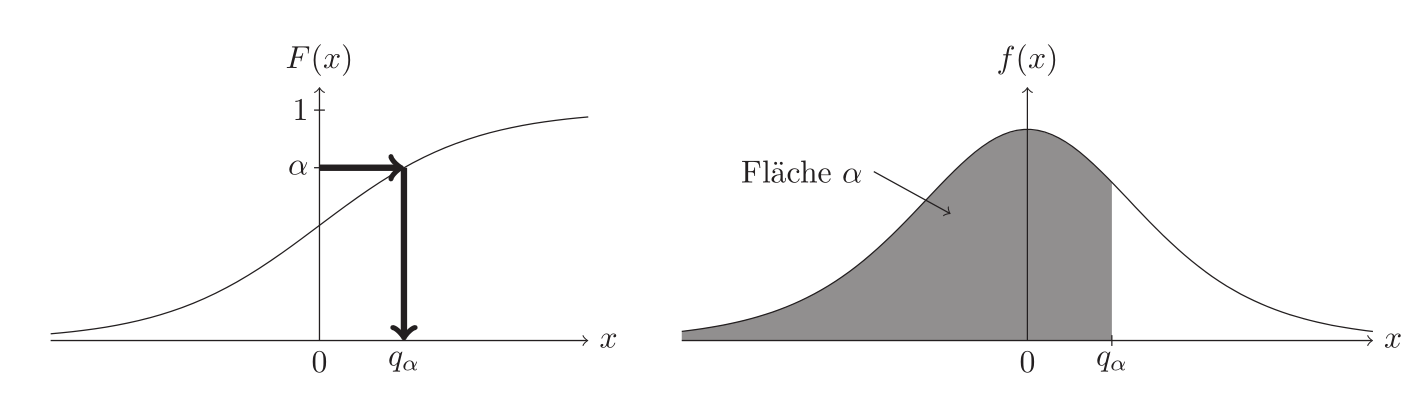
\includegraphics[width=0.8\linewidth]{img/quantile}
\end{center}


\end{document}
